
This lecture covers disturbances in electircal circuits, such as common mode
current, Electro Magnetic Pulses and Electro Static Discharge. Distrurbances are
gathered under the name Electro Magnetic Interference, or \textit{EMI}, and the
amount of EMI a circuit generates is related to Electro Magnetic Compatibility,
\textit{EMC}. A good EMC means low or no interference. 
\newline
EMP occurs during lightning strikes and nuclear blasts. The power of an EMP
blast is very high but only lasts around 50 $\mu$s and does as such not contain much
energy. 
\subsubsection*{EMC Characteristics}
EMC can be transferred to and from a system in two ways, radiation and
conduction. A systems EMC characteristics are therefore divided into Radiated
Emission (RE) and Radiated Immunity (RI) as well as Conducted Immunity (CI) and
Conducted Emission (CE). The frequencies of these emissions and immunities have
shifted over the years to a point where both emission and the receptability of
disturbances are now in the same area. This is described called the
\textit{Compatibility funnel}.
\subsubsection*{Signal traces}
A circuit with contains a changing current becomes an antenna, emitting electro
magnetic waves. There are several types of antenna, three of wich are shown
below. 
% Three figures of antennas
\begin{figure}[H]
\centering
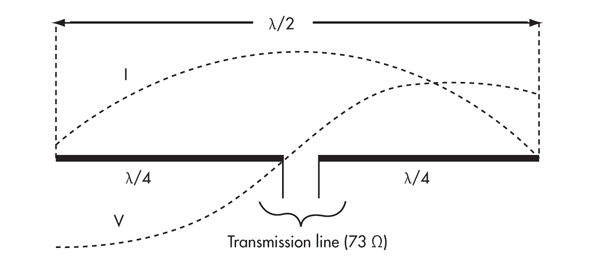
\includegraphics{./figures/FIG_dipoleantenna.png}
\caption{A dipole antenna.}
\ref{fig:dipoleantenna}
\end{figure}
\begin{figure}[H]
\centering
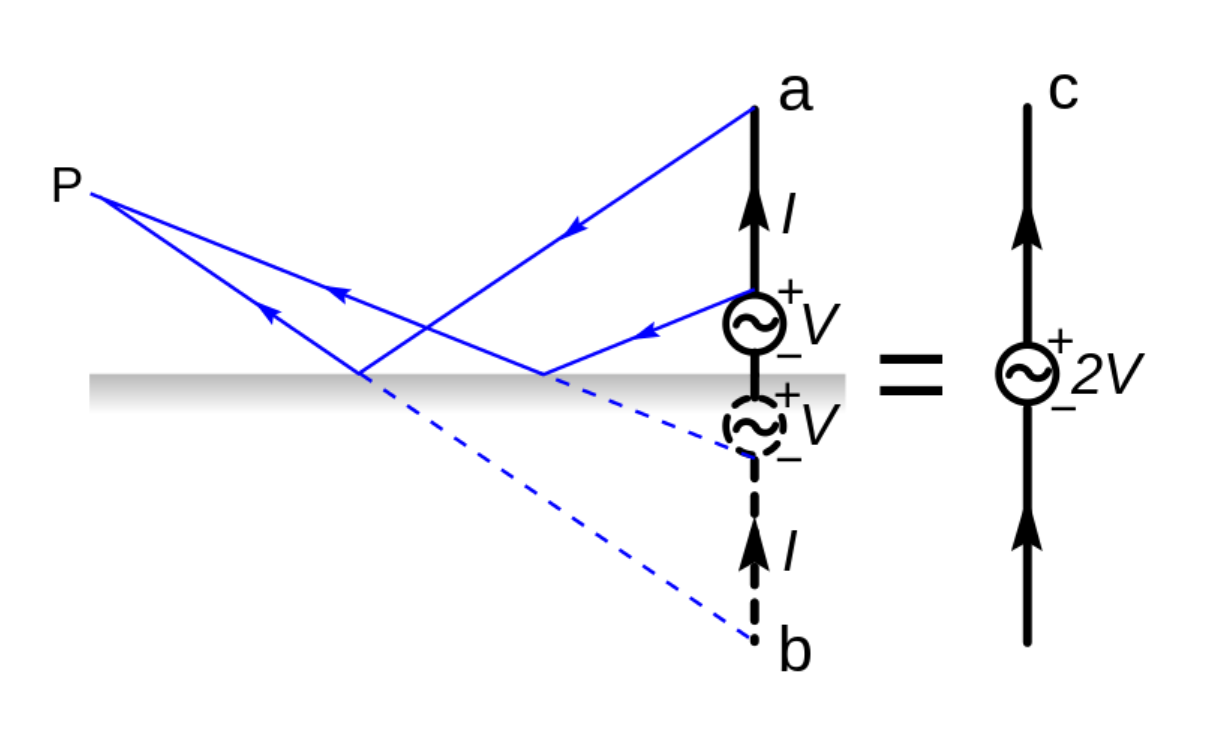
\includegraphics[scale=0.3]{./figures/FIG_rodantenna.png}
\caption{A rod antenna.}
\ref{fig:rodantenna}
\end{figure}
\begin{figure}[H]
\centering
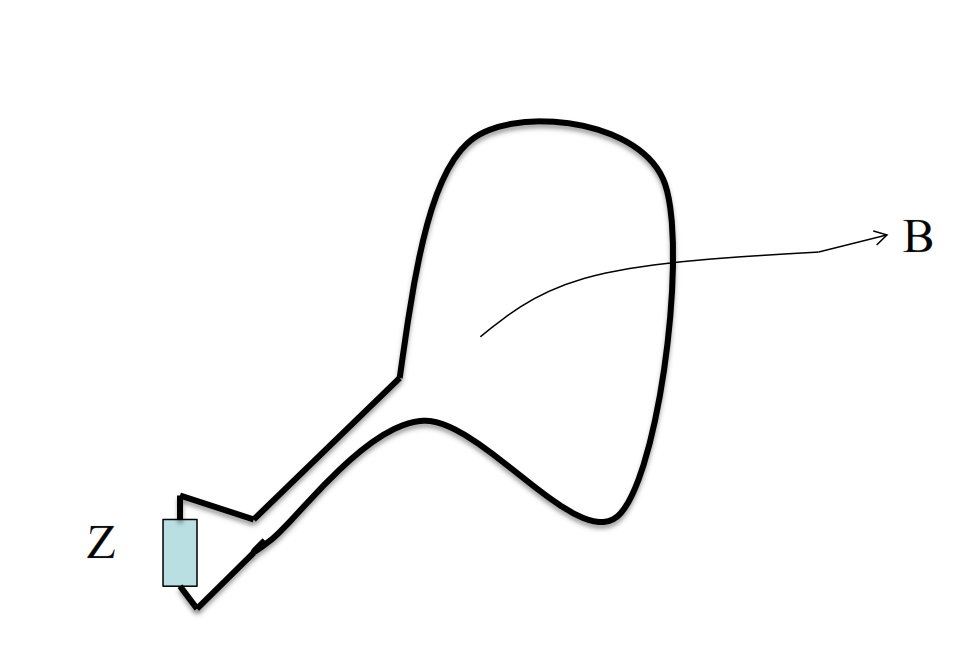
\includegraphics[scale=0.3]{./figures/FIG_loopantenna.png}
\caption{A loop antenna.}
\ref{fig:loopantenna}
\end{figure}
If a the layout of a circuit is not designed properly, it might exhibit antenna
like behaviour, leading to EMI. Especially loop antenna phenomenon are common in
parts of a closed circuit where current is alternating frequently but there are
also examples of dipole antenna behaviour. In general, it is desired to let the
return current be able to run directly underneath the feed current line. This is
what the current will do unless hindered. Figure~\ref{fig:pcbcrossantenna}
displays a two-layer board where the return current is forced to take a longer
return route, causing a loop antenna and therefore reducing its EMC.
\begin{figure}[H]
\centering
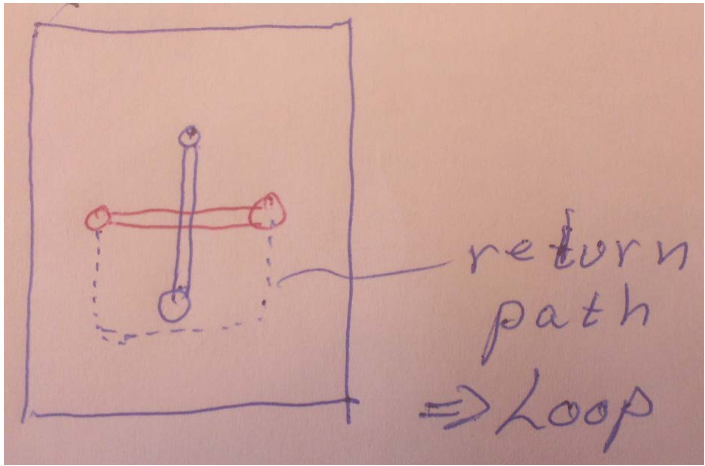
\includegraphics[scale=0.7]{./figures/FIG_pcbcrossantenna}
\caption{A loop antenna in a two-layer PCB.}
\ref{fig:pcbcrossantenna}
\end{figure}
The best solution is to not cut in the ground plane, thus leaving the return
paths as untouched as possible. It is also important to avoid sharp edges in the
signal trace since this causes reflection and radiation. 
\subsubsection*{Coupling modes}
The voltage differences within a circuit are called \textit{Differential mode}
voltages. These are normal and cause the current to flow in the closed circuit.
When the voltages within the circuit change together is called \textit{Common
mode}. This causes the current to flow in the same direction in all cables and
is present even when there is no visible connection to the surroundings. Common
and differential modes is displayed in Figure~\ref{fig:couplingmodes}.
\begin{figure}[H]
    \centering
    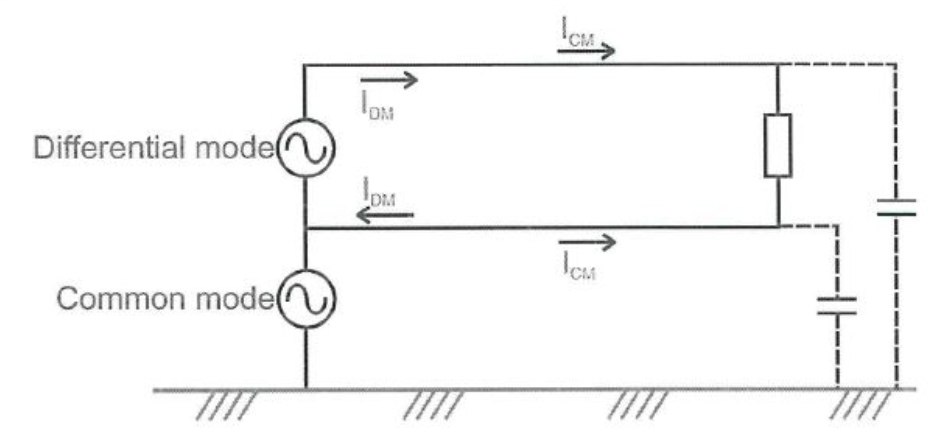
\includegraphics[scale=0.7]{./figures/FIG_couplingmodes.png}
    \caption{Different coupling modes.}
    \ref{fig:couplingmodes}
\end{figure}
Because the common mode current is dependant on the common mode impedance,
sometimes grounding is not desired since a lower impedance causes a higher
current. This is demonstrated in Figure~\ref{fig:commongrounding}.
% Impedance when grounding a cable
\begin{figure}[H]
\centering
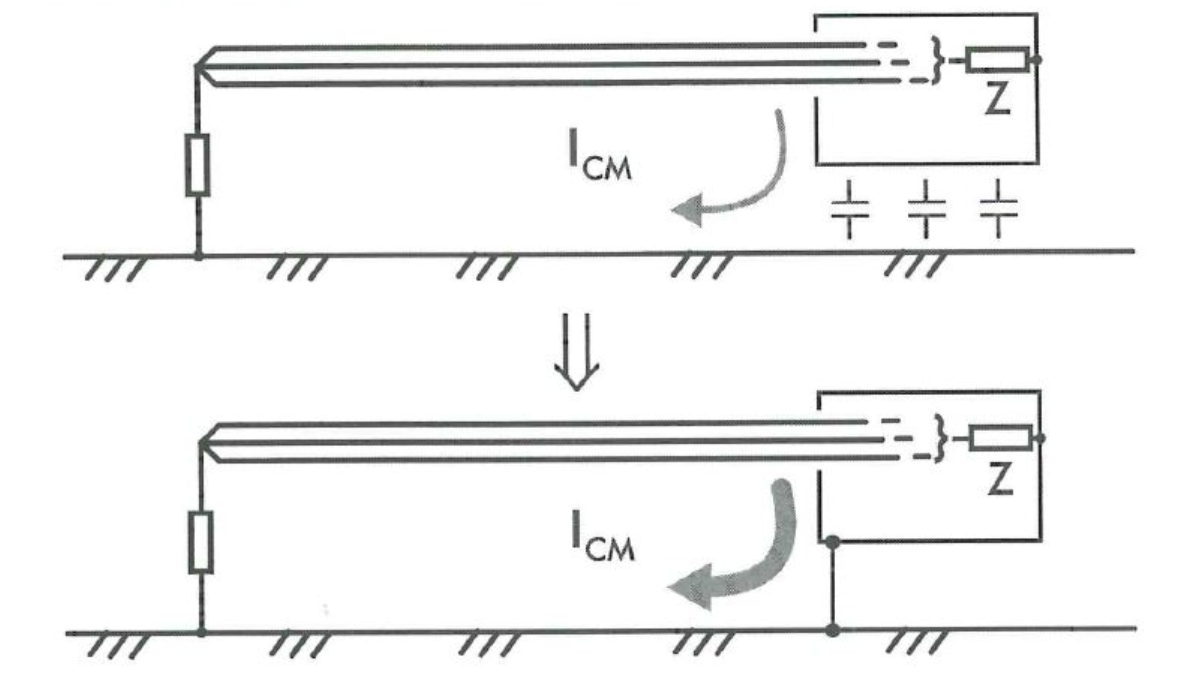
\includegraphics[scale=0.7]{./figures/FIG_commongrounding.png}
\caption{Different coupling modes.}
\ref{fig:couplingmodes}
\end{figure}
When calculating the interference the common mode current has on the
differential mode current, the model in
Figure~\ref{circ:commonimpedancecoupling} is useful.
% Common impedance coupling scheme
\begin{figure}[H]
\centering
\begin{circuitikz}[scale=1] \draw
    (0,0) node[ground] {A}
        to [short, -*] (0,2)
        to [european voltage source] (0,6)
        to [R, R=$R_{out}$] (3,6)
        to [R, R=$Z_w$] (10,6)
        to [R, R=$R_{in}$, -*, v=$U_{DM}$] (10,2)
        -- (10,0) node[ground] {B}
        to [R, R=$Z_g$, v=$U_{AB}$] (3,0)
        -- (0,0)
    (0,2) -- (3,2)
        to [R, R=$Z_w$] (10,2)

;
\end{circuitikz}
\label{circ:commonimpedancecoupling}
\end{figure}

For the interference, the following equation is true,
% Equation for common impedance coupling
\begin{equation}
    U_{DM} = \frac {U_{CM}R_{in}} {R_{out} + R_{in}}.
    \label{eq:udminterference}
\end{equation}

\begin{example}
    For a circuit as in with
    \begin{itemize}
        \item $R_{in}=1\si{\mega\ohm}$
        \item $R_{out}=1\si{\kilo\ohm}$
        \item $U_{CM}=0.1\si{V}$
    \end{itemize}
    The Differential mode interference is
    \begin{flalign*}
        U_{DM}= \frac {U_{CM}R_{in}} {R_{out} + R_{in}} = \frac {0.1\cdot1}
        {\num{1e3}\cdot\num{1e6}}=0.1\si{V}
    \end{flalign*}
\end{example}



